\subsection{Neighbour Pruning Rules} 
\label{sec:pruning}

In this section we develop rules for pruning the set of nodes immediately 
adjacent to some node $x$ from the grid.
The objective is to identify from each
set of such neighbours, i.e. $neighbours(x)$, any nodes $n$ that do not need to be evaluated in order to
reach the goal optimally. We achieve this by comparing the length of two paths:
$\pi$, which begins with node $p(x)$ visits $x$ and ends with $n$ and another
path $\pi'$ which also begins at node $p(x)$ and ends with $n$ but does not 
mention $x$. 
Additionally, each node mentioned by either $\pi$ or $\pi'$ must belong to 
$neighbours(x)$.
There are two cases to consider, depending on
whether the transition to $x$ from its parent $p(x)$ involves a straight move or
a diagonal move. 

\begin{figure}[h]
       \begin{center}
		   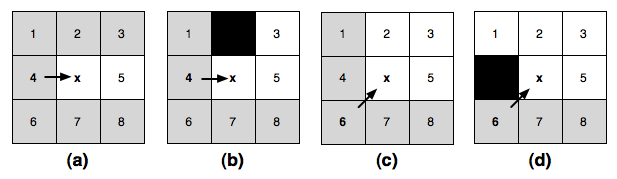
\includegraphics[scale=0.4, trim = 10mm 10mm 10mm 0mm]
			{diagrams/pruningrules.png}
       \end{center}
	\vspace{-3pt}
       \caption{We show several cases where a node $x$ is reached from its
parent $p(x)$ by either a straight or diagonal move. When $x$ is expanded we can
prune from consideration all nodes marked grey.}
       \label{fig:pruning}
\end{figure}
\par \noindent
\textbf{Straight Moves:} We prune any node $n \in neighbours(x)$ which 
satisfies the following dominance constraint:
\begin{equation}
len(~<p(x), \ldots, n> \setminus x~)
\leq len(~<p(x), x, n >~)
\end{equation}
Figure \ref{fig:pruning}(a) shows an example. Here $p(x) = 4$ and we prune
 all neighbours except $n = 5$.
%In some cases we may be \emph{forced} to evaluate a neighbour which would be
%dominated except for the presence of obstacles that are adjacent to $x$.  We
%show an example of this situation in Figure \ref{fig:pruning}(b); notice that 
%in addition to $n = 5$ we are also forced to consider $n = 3$. 
\par \noindent
\textbf{Diagonal Moves:} This case is similar to the pruning rules we developed
for straight moves; the only difference is that the path which excludes $x$ must 
be strictly dominant: 
\begin{equation}
len(~<p(x), \ldots, n> \setminus x~) < len(~<p(x), x, n>~)
\end{equation}
Figure \ref{fig:pruning}(c) shows an example. Here $p(x) = 6$ and we prune all
neighbours except $n = 2$, $n = 3$ and $n = 5$.  
%As before when $x$ is adjacent
%to an obstacle we may be forced to evaluate additional neighbours. For example
%in Figure \ref{fig:pruning} the evaluation of node $n = 1$ is forced.
\par
Assuming $neighbours(x)$ contains no obstacles, we will refer to the nodes
that remain after the application of straight or diagonal pruning (as
appropriate) as the \emph{natural neighbours} of $x$. These correspond to the non-gray
nodes in Figures \ref{fig:pruning}(a) and \ref{fig:pruning}(c).
When $neighbours(x)$ contains an obstacle, we may not be able to prune
all non-natural neighbours. If this occurs we say that the evaluation of each
such neighbour is \emph{forced}.

\begin{definition}
\label{def:forced}
A node $n \in neighbours(x)$ is forced if: \\
\indent
1. $n$ is not a natural neighbour of $x$\\
\indent
2. $ len(~< p(x), x, n >~) < len(~ < p(x), \ldots, n > \setminus x~)$
\end{definition}
\par \noindent
In Figure \ref{fig:pruning}(b) we show an example of a straight move where 
the evaluation of $n = 3$ is forced. Figure \ref{fig:pruning}(d)  
shows an similar example involving a diagonal move; here the evaluation of
$n = 1$ is forced.
